\begin{center}
    \captionof{figure}{Within- and Between-Person Effects of Continuous Predictor and Dichotomous Outcome}

    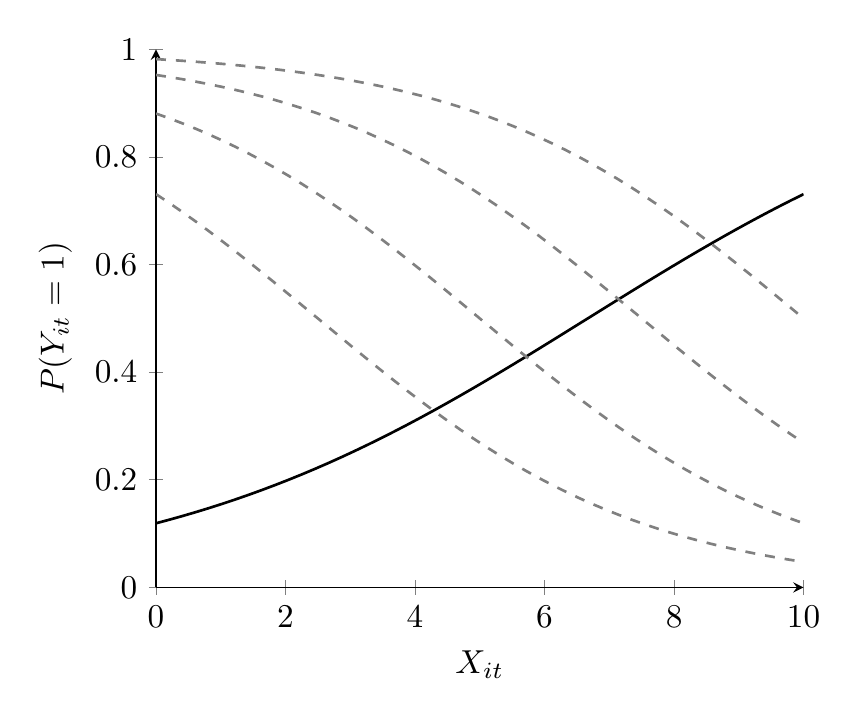
\begin{tikzpicture}[scale=1.2]
    \begin{axis}[
        axis x line=left, 
        axis y line=left, 
        % width=10cm, height=8cm,
        xlabel={$X_{it}$}, ylabel={$P(Y_{it} = 1)$},
        ymin=0, ymax=1, xmin=0, xmax=10,
        % legend pos=north west
    ]

    % Define parameters
    \pgfmathsetmacro{\intercept}{-2}  % Logit-scale intercept
    \pgfmathsetmacro{\slopeB}{0.3}     % Between effect in logit space
    \pgfmathsetmacro{\slopeW}{-0.4}    % Within effect in logit space

    % Between-person effect (blue solid line)
    \addplot[black, thick, domain=0:10, samples=50] 
        {1 / (1 + exp(-(\intercept + \slopeB*x)))};
    % \addlegendentry{Between-person effect}

    % Within-person effect (red dashed line)
    \addplot[gray, thick, dashed, domain=0:10, samples=50] 
        {1 / (1 + exp(-(\intercept + 3 + (\slopeW)*x)))};
    \addplot[gray, thick, dashed, domain=0:10, samples=50] 
        {1 / (1 + exp(-(\intercept + 4 + (\slopeW)*x)))};
    \addplot[gray, thick, dashed, domain=0:10, samples=50] 
        {1 / (1 + exp(-(\intercept + 5 + (\slopeW)*x)))};
    \addplot[gray, thick, dashed, domain=0:10, samples=50] 
        {1 / (1 + exp(-(\intercept + 6 + (\slopeW)*x)))};

    \end{axis}
\end{tikzpicture}

    \label{fig:withinbetween-contxbiny}
    \begin{figurenote}
        The solid black slope represents the between-person effect and the dashed solid grey slopes the within-cluster effects. The X-axis simultaneously represents $X_{it}$ for the within-slope and $\mu_{X,i}$ for the between-slope.
    \end{figurenote}
\end{center}

